\def\year{2015}
\documentclass[letterpaper]{article}

\usepackage{aaai}
\usepackage{times}
\usepackage{helvet}
\usepackage{courier}

\usepackage{graphicx}
\usepackage{amsmath}
\usepackage{amssymb}
\usepackage{amsthm}

\frenchspacing
\setlength{\pdfpagewidth}{8.5in}
\setlength{\pdfpageheight}{11in}

\pdfinfo{
/Title (Insert Your Title Here)
/Author (Put All Your Authors Here, Separated by Commas)}

\setcounter{secnumdepth}{0}  

% We define our own macros here
\newcommand{\mat}[1]{\mathbf{#1}}
\newcommand{\A}{\mat{A}}
\newcommand{\B}{\mat{B}}
\newcommand{\M}{\mat{M}}
\newcommand{\Rset}{\mathbb{R}}
\newcommand{\Nset}{\mathbb{N}}
\newcommand{\Hset}{\mathbb{H}}
\newcommand{\pivec}{\boldsymbol{\pi}}
\newcommand{\alphavec}{\boldsymbol{\alpha}}
\newcommand{\thetavec}{\boldsymbol{\theta}}
\newcommand{\rhovec}{\boldsymbol{\rho}}
\newcommand{\vecalpha}{\alphavec}
\newcommand{\vectheta}{\thetavec}
\newcommand{\vecrho}{\rhovec}
\newcommand{\aone}{\boldsymbol{\alpha}_\lambda}
%\newcommand{\aone}{\boldsymbol{\alpha}_0}
\newcommand{\ainf}{\boldsymbol{\alpha}_{\infty}}
\newcommand{\taone}{\tilde{\boldsymbol{\alpha}}_0}
\newcommand{\tainf}{\tilde{\boldsymbol{\alpha}}_{\infty}}
\newcommand{\haone}{\hat{\boldsymbol{\alpha}}_0}
\newcommand{\hainf}{\hat{\boldsymbol{\alpha}}_{\infty}}
\newcommand{\bone}{\boldsymbol{\beta}_0}
\newcommand{\binf}{\boldsymbol{\beta}_{\infty}}
\newcommand{\vecb}{\boldsymbol{\beta}}
\newcommand{\tbone}{\tilde{\boldsymbol{\beta}}_0}
\newcommand{\tbinf}{\tilde{\boldsymbol{\beta}}_{\infty}}
\newcommand{\hbone}{\hat{\boldsymbol{\beta}}_0}
\newcommand{\hbinf}{\hat{\boldsymbol{\beta}}_{\infty}}
\newcommand{\Alpha}{\aone}
\newcommand{\Beta}{\ainf}
\newcommand{\psrA}{\mathcal{A}}
\newcommand{\psr}{\langle  \aone, \ainf, \{\A_\sigma\} \rangle}
\newcommand{\psrsigma}{\langle \Sigma, \aone, \ainf, \{\A_\sigma\}_{\sigma \in \Sigma} \rangle}
\newcommand{\mpsrsigma}{\langle \Sigma, \Sigma', \kappa, \aone, \ainf, \{\A_\sigma\}_{\sigma \in \Sigma'} \rangle}

%\newcommand{\wb}{\langle  \bone, \binf, \{\B_\sigma\} \rangle}
%\newcommand{\wap}{\langle  \aone', \ainf', \{\A'_\sigma\} \rangle}
%\newcommand{\wbp}{\langle  \bone', \binf', \{\B'_\sigma\} \rangle}
%\newcommand{\wat}{\langle  \taone, \tainf, \{\tilde{\A}_\sigma\} \rangle}
%\newcommand{\wtt}{\langle  \taone, \tainf, \{\tilde{\A}_\sigma^\delta\} \rangle}
%\newcommand{\wt}{\langle  \aone, \ainf, \{{\A}_\sigma^\delta\} \rangle}
%\newcommand{\wbt}{\langle  \tbone, \tbinf, \{\tilde{\B}_\sigma\} \rangle}
%\newcommand{\wah}{\langle  \haone, \hainf, \{\hat{\A}_\sigma\} \rangle}
%\newcommand{\wbh}{\langle  \hbone, \hbinf, \{\hat{\B}_\sigma\} \rangle}


\begin{document}

\title{TITLE GOES HERE}
\author{Anonymous Submission}
\maketitle

\begin{abstract}
\begin{quote}
Fancy Abstract...
\end{quote}
\end{abstract}

\section{Introduction}

Learning models of partially observable dynamical systems is very important in practice --- several alternatives...

General algorithms are not designed to exploit frequen patterns/structure in sequences of observations to speed-up learning --- but in practice with large observations and highly structured environments this might be necessary to achieve decent results

We propose a new model of predictive state representation for environments with discrete observations: the multi-step PSR (M-PSR)

We show how the standard spectral learning for PSR extends to M-PSR

Then we present a data-driven algorithm for selecting a particular M-PSR from data sampled from a structured partially observable environment

We evaluate the performance of our algorithms in an extensive collection of synthetic environments and conclude that...

\section{M-PSR: Definition and Learning}

\subsection{Multi-Step PSR}

A linear \emph{predictive state representation} for an autonomous dynamical system with discrete observations in a set $\Sigma$ is a tuple $\psrA = \psrsigma$ where: BLA BLA.

To define our model for multi-step PSR we basically augment a PSR with two extra objects: a set of \emph{multi-step observations} $\Sigma' \subset \Sigma^+$ containing non-empty strings formed by basic observations, and a \emph{coding function} $\kappa : \Sigma^\star \to {\Sigma'}^{\star}$ that given a string of basic observations produces an equivalent string composed using multi-step observations.
%
The choice of $\Sigma'$ and $\kappa$ can be quite application-dependent, in order to reflect the particular patterns arising from different environments. However, we assume this objects satisfy a basic set of requirements for the sake of simplicity and to avoid degenerate situations:
\begin{enumerate}
\item The set $\Sigma'$ must contain all symbols in $\Sigma$; i.e.\ $\Sigma \subseteq \Sigma'$
\item The function $\kappa$ satisfies $\partial(\kappa(x)) = x$ for all $x \in \Sigma^\star$, where $\partial : {\Sigma'}^\star \to \Sigma^\star$ is the \emph{decoding morphism} between free monoids given by $\partial(z) = z \in \Sigma^\star$ for all $z \in \Sigma'$. Note this implies that $\kappa(\epsilon) = \epsilon$, $\kappa(\sigma) = \sigma$ for all $\sigma \in \Sigma$, and $\kappa$ is injective.
\end{enumerate}

Using these definitions, a \emph{multi-step PSR} (M-PSR) is a tuple $\psrA' = \mpsrsigma$.

\subsection{Spectral Learning Algorithm}

We extend \cite{bootspsr}...

\subsection{Examples}

%\textbf{Base PSR for Duration Models} BLA BLA...

In this section we will go through a few examples of Multi-PSRs which are particularly relevant to our experiment section. 

For the timing case one can use a M-PSR which we call the \textbf{Base System}. For this type of M-PSR, $\sum'$ will consist of $\{a^{2^k} \forall k <= n\}$. To describe the encoding map we write an observation $a^m = a^{2^n1} ... \cdot a^{2^nf}$  With this equality a natural encoding map $\kappa$ which is natural to use is: $\kappa(a^n) = \{a^{2^n_1},...,\{a^{2^n_f}\}$. 

For the multiple observation case one can also use The Base System. In this case $\sum' = \{\sigma^{2^k}\forall \sigma \in \sum, \forall k <= n\}$. For the encoding map $\kappa$ we first split the string into sequences of a fixed symbol and then use the same encoding as for timing. The Base System for multiple observations clearly aims at environments where observation symbols come in streaks.
 
Another example for the multiple observation case is an M-PSR we will call the \textbf{Tree System}. For the Tree System, we set $\sum'=$ the set of all possible strings of length $<= L$. For the decoding map $\kappa$, we first split a string x into $x_1x_2...x_ny$, where $xi$ $\forall i<=n$ have length L and y has length $len(x) - n \times L$. With this we set $\kappa(x) = \{x_1,x_2,...,y\}$.

The the construction of the above multi-PSRs is not dependent on the environment. In practice, if one would like to learn a M-PSR which has the best performance, namely a M-PSR whose parameters best reflect the types of observations seen from one's environment. 

\section{Fully Data-Driven Learning}

\subsection{Learning Transition Operators}

Here we present a greedy heuristic which learns our transition sequences $\sum'$ from observation data. We start with some notation. Let ... 

ALGORITHM CODE:

\subsection{Learning the encoding function}

Here we provide a dynamic programming algorithm which can serve as $kappa$ for any M-PSR. Given a query string Q, and a set of transition sequences $\sum'$, the algorithm minimizes the number of sequences used in the partition. In other words, the algorithm minimizes $|k(Q)|$.

ALGORITHM CODE:


\section{Experiments}

We assess the performance of the Base System on labyrinth environments. The robot is positioned in a starting location and it stochastically navigates the environment. We split the experiments into two cases. The first is the case of timing, where $\sum = \{\sigma\}$ and the second is with multiple observations. For timing, the goal is to make predictions about how long the agent will survive the environment. One can also ask conditional queries such as how long the agent should expect to survive given that x seconds have elapsed. For multiple observations we place the agent in the environment, let it roam for a fixed time length and then remove the agent. The goal for the multiple observation labyrinth will be to make predictions about seeing observation sequences. In both cases, we analyse the performance for PSRs of different model sizes with a fixed observation set. For each Base System PSR, we include all powers of 2 up to 256. For the heuristic based PSRs we learn 10 operators from the observations with the greedy algorithm described in (). To measure the performance of a PSR we use the following norm:
$||f - \hat{f}|| = \sqrt{\sum\nolimits_{x \in observations}(f(x) - \hat{f(x)})^2}$. We use this norm because of a bound presented by [AUTHORS], which states that (). 

\subsection{Learning PSRs for Timing}
For the timing case, we construct our empirical hankel matrix by including ${\sigma^i i<=n}$. With this choice, the empirical hankel matrix will be a nxn matrix with the prefixes and suffixes being the same.The parameter n depends on the application. For Double Loop environments we set n to be 300, while for pacMan it was 600. The important  property that needs to be satisfied when choosing the parameter n is that enough observations are captured to learn a good model. Something here: $\lim_{ \to 2} f(x) = 5$ .

\subsection{Learning PSRs for Multiple Observations}

For multiple observations a slightly more complex approach is required to construct the empirical hankel matrix. For prefixes, we select the k most frequent prefixes from our observations set. For suffixes we take all suffixes that occur from our set of prefixes. This heuristic was given in previous work by [] and it showed that ().


\subsection{Double Loop Timing}

For timing, we start by considering a double loop environment. The agent starts at the intersection of the two loops. At the intersection, the agent has a 50 percent chance of entering either loop. Exit states are located halfway between each loop. At an exit state, the agent has a 50 percent probability of exiting the environment. Observations are generated by placing the agent in the environment: $\sigma^{100}$ corresponds to the agent surviving 100 time units. In figure 1, we learn a PSRs with 10000 observation sequences. We generate 10 PSRs and average their performance. 

\begin{figure}[ht!]
\centering
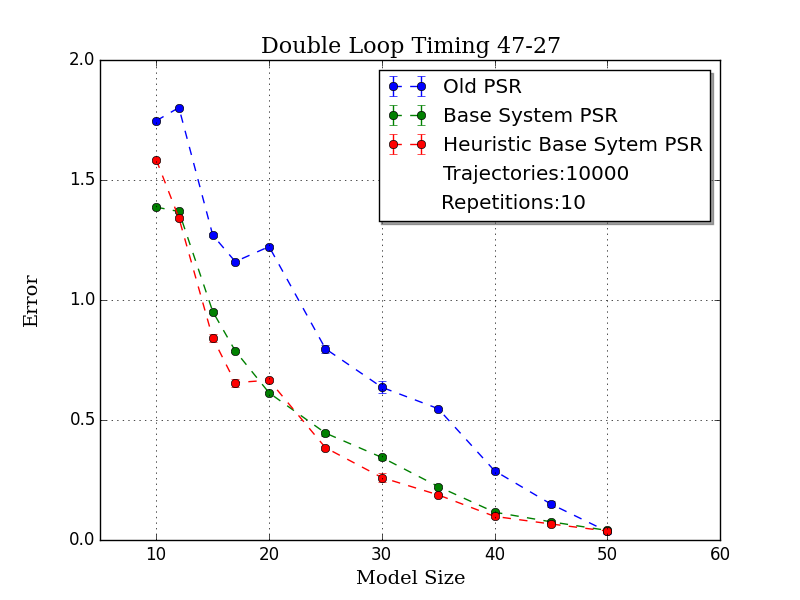
\includegraphics[width=60mm]{uCOREPICS/DoubleLoopTimingHeuristics47-27.png}
\caption{Double Loop Environment\label{overflow}}
\end{figure}

\begin{figure}[ht!]
\centering
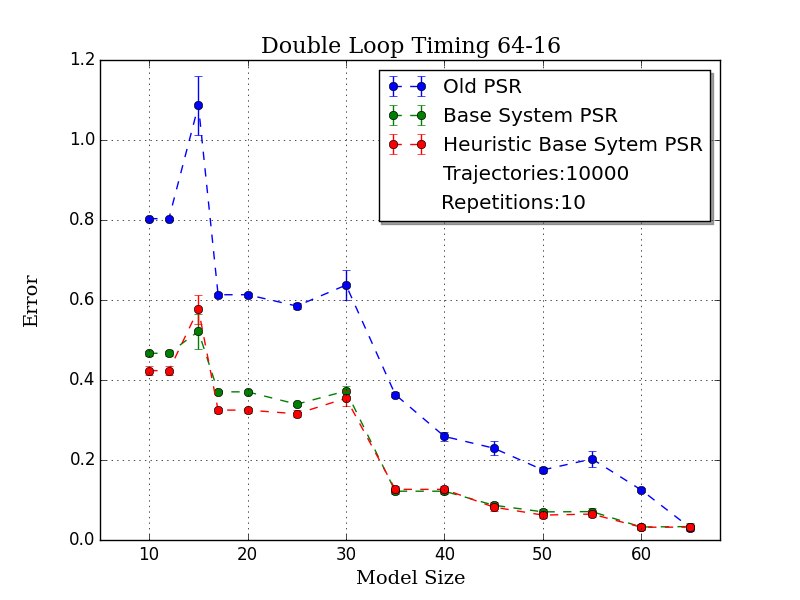
\includegraphics[width=60mm]{uCOREPICS/DoubleLoop64-16Heuristics.png}
\caption{Double Loop Environment\label{overflow}}
\end{figure}

\subsection{Pacman Timing}

We proceed to work with timing in a Pacman environment. The transition structure of this environment is shown in Figure 2. Edge weights vary from 1 to 3 and are stretched by a parmater we call the stretch factor which we initialize at 10. Again we use 10000 observation sequences per PSR and compute the average of 10 PSRs.

\begin{figure}[ht!]
\centering
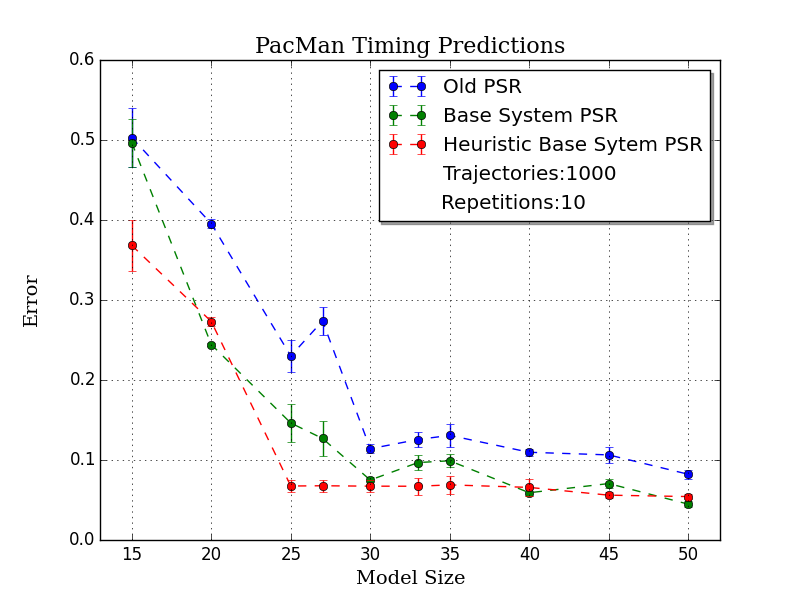
\includegraphics[width=60mm]{uCOREPICS/PacManTimingHeuristicsIncluded.png}
\caption{Double Loop Environment\label{overflow}}
\end{figure}

\subsection{Timing - Results}
As is demonstrated in figure 3, learning longer transitions provides a significant improvement over the standard for truncated models. The heuristic based approach performs slightly better than the powers of two method. For the double loop case the heuristic approach learns multiples of the loop lengths which results in partitions which use fewer operators. For Pacman, the operators that are learned are various multiples of the stretch factor, which once again shows that the greedy heuristic is effective. 

\subsection{Multiple Observations}

To test whether the Base System would translate to multiple observations we construct a double loop environment where one loop is green and the other is blue. The lengths of each loop are also varied. We fix the length of observations to be $loop1 + loop2 * 3$. To build empirical estimates of probabilities we set f(x)=prefix-occ(x)/num-strings-length>=x.

\subsection{Multiple Observations Results}

\begin{figure}[ht!]
\centering
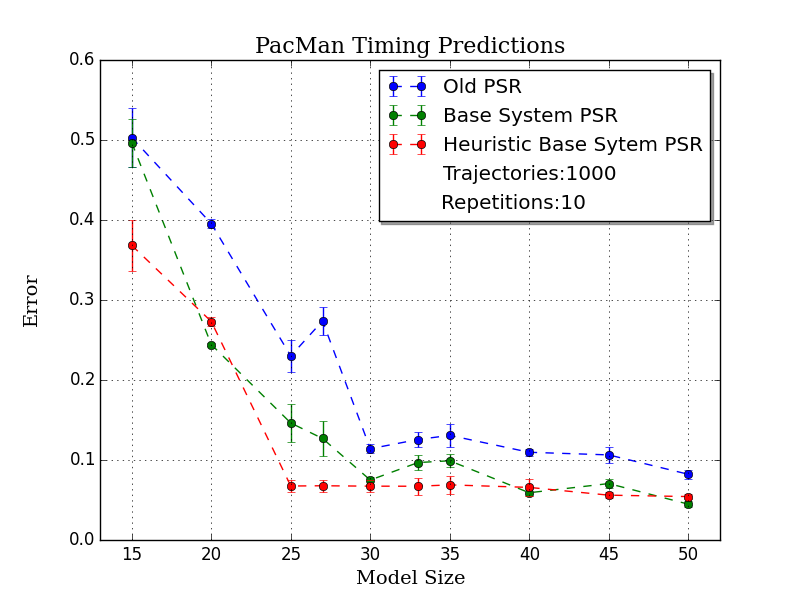
\includegraphics[width=60mm]{uCOREPICS/PacManTimingHeuristicsIncluded.png}
\caption{Double Loop Environment\label{overflow}}
\end{figure}

\section{Conclusion}

\section{Acknowledgments}
Funding and friends...

\bibliographystyle{aaai}
\bibliography{references}

\end{document}
